\section{Aplikasi Op-Amp}

\subsection{Pengantar Aplikasi Op-Amp}
\begin{frame}{Pengantar Aplikasi Op-Amp}
	\begin{itemize}
		\item Aplikasi dari op amp sangat luas sekali dan beraneka ragam
		\item Tidak mungkin menjelaskannya secara komprehensif
		\item Sementara kita fokus pada 2 rangkaian dulu.
	\end{itemize}
\end{frame}

\subsection{The Summing Amplifier}
\begin{frame}{The Summing Amplifier}
	\begin{multicols}{2}
		\begin{figure}
			\centering
			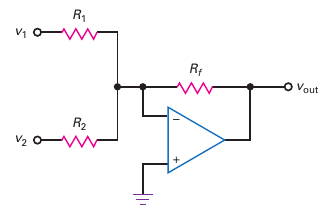
\includegraphics[width=0.9\linewidth]{gambar/fig-16.23a}
			\caption{Rangkaian umming amplifier}
			\label{fig-16.23a}
		\end{figure}
		\begin{itemize}
			\item Menggabungkan 2 atau lebih sinyal analog menjadi satu output
		\end{itemize}
		\columnbreak
		\begin{itemize}
			\item Menguatkan setiap sinyal input
			\item Penguatan setiap channel atau input
			\begin{align*}
				A_{v1(CL)} = \frac{-R_f}{R_1};~~ A_{v2(CL)} = \frac{-R_f}{R_2}
			\end{align*}
			\item Tegangan output
			\begin{equation}\label{pers.16.13}
				v_{out} = A_{v1(CL)}v_1 + A_{v2(CL)} v_2
			\end{equation}
			\item Resistor Thevenin:
			\begin{equation}
				R_{B2} = R_1 \parallel R_2 \parallel R_f \parallel \cdots \parallel R_n
			\end{equation}
		\end{itemize}
	\end{multicols}
\end{frame}

\begin{frame}{The Summing Amplifier}
	\begin{multicols}{2}
		\begin{figure}
			\centering
			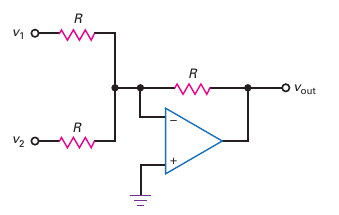
\includegraphics[width=\linewidth]{gambar/fig-16.23b}
			\caption{Rangkaian summing amplifier dengan resistor yang sama}
			\label{fig-16.23b}
		\end{figure}
		\columnbreak
		\begin{itemize}
			\item Tegangan output
			\begin{equation*}
				v_{out} = -(v_1 + v_2 + \cdots + v_n)
			\end{equation*}
		\end{itemize}
	\end{multicols}
\end{frame}

\begin{frame}{The Summing Amplifier}
	\begin{multicols}{2}
		\begin{figure}
			\centering
			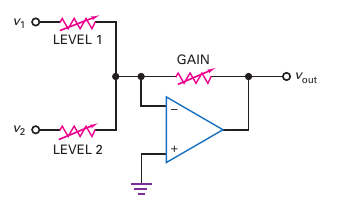
\includegraphics[width=\linewidth]{gambar/fig-16.23c}
			\caption{Rangkaian mixer}
			\label{fig-16.23c}
			\columnbreak
			\begin{itemize}
				\item Menggabungkan sinyal audio
				\item Menurunkan LEVEL 1 $ \rightarrow $ sinyal $ v_1 $ semakin nyaring di output
				\item Menurunkan LEVEL 2 $ \rightarrow $ sinyal $ v_2 $ semakin nyaring di output
				\item Meningkatkan GAIN $ \rightarrow $ kedua sinyal semakin nyaring
			\end{itemize}
		\end{figure}
	\end{multicols}
\end{frame}

\subsection{Voltage Follower}
\begin{frame}{Voltage Follower}
	\begin{multicols}{2}
		\begin{figure}
			\centering
			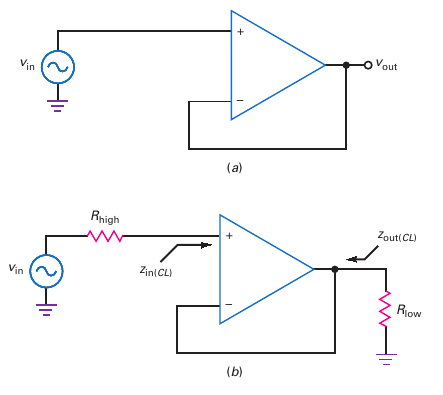
\includegraphics[width=0.9\linewidth]{gambar/fig-16.24}
			\caption{Rangkaian voltage follower}
			\label{fig-16.24}
		\end{figure}
		\columnbreak
		\begin{itemize}
			\item Penguatan tegangan closed-loop:
			\begin{equation}\label{pers.16.15}
				A_{v(CL)} = 1
			\end{equation}
			\item Bandwidth closed-loop:
			\begin{equation}\label{pers.16.16}
				f_{2(CL)} = f_{unity}
			\end{equation}
		\end{itemize}
	\end{multicols}
\end{frame}

\subsection{Contoh Soal 2.12}
\begin{frame}{Contoh Soal 2.12}
	\begin{multicols}{2}
		\begin{center}
			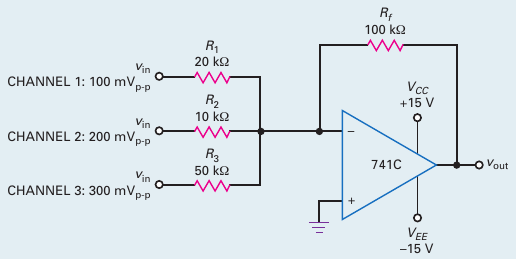
\includegraphics[width=\linewidth]{gambar/fig-16.25}
		\end{center}
		\columnbreak
		\begin{itemize}
			\item Pertanyaan:
			\begin{itemize}
				\item Berapa tegangan output ac?
			\end{itemize}
			\item Jawaban:
			\begin{itemize}
				\item Penguatan tegangan tiap channel:
				\begin{align*}
					A_{v1(CL)} &= \frac{-R_f}{R_1} = \frac{-100 \text{ k}\Omega}{20 \text{ k}\Omega} = -5 \\
					A_{v2(CL)} &= \frac{-R_f}{R_2} = \frac{-100 \text{ k}\Omega}{10 \text{ k}\Omega} = -10 \\
					A_{v3(CL)} &= \frac{-R_f}{R_3} = \frac{-100 \text{ k}\Omega}{50 \text{ k}\Omega} = -2 \\
				\end{align*}
			\end{itemize}
		\end{itemize}
	\end{multicols}
\end{frame}

\begin{frame}{Contoh Soal 2.12}
	\begin{multicols}{2}
		\begin{center}
			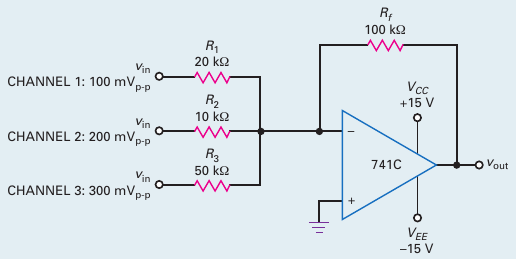
\includegraphics[width=\linewidth]{gambar/fig-16.25}
		\end{center}
		\columnbreak
		\begin{itemize}
			\item Jawaban:
			\begin{itemize}
				\item Tegangan output:
				\begin{align*}
					v_{out} = A_{v1(CL)} v_1 + A_{v2(CL)} v_2 + A_{v3(CL)} v_3
				\end{align*}
				\item Jika diperlukan untuk mengkompensasi bias input dengan menambahkan $ R_B $ yang sama ke noninverting input
				\begin{align*}
					R_{B2} &= R_1 \parallel R_2 \parallel R_3 \parallel R_f \\
					&= 20 \text{ k}\Omega \parallel 10 \text{ k}\Omega \parallel 50 \text{ k}\Omega \parallel 100 \text{ k}\Omega \\
					&= 5.56 \text{ k}\Omega
				\end{align*}
			\end{itemize}
		\end{itemize}
	\end{multicols}
\end{frame}

\subsection{Latihan Soal 2.12}
\begin{frame}{Latihan Soal 2.12}
	\begin{multicols}{2}
		\begin{center}
			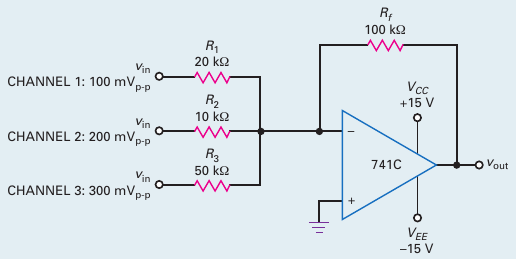
\includegraphics[width=\linewidth]{gambar/fig-16.25}
		\end{center}
		\columnbreak
		\begin{itemize}
			\item Pertanyaan:
			\begin{itemize}
				\item Jika tegangan input peak-to-peak diganti dengan tegangan positif dc, berapakah tegangan output dc-nya?
			\end{itemize}
		\end{itemize}
	\end{multicols}
\end{frame}

\subsection{Contoh Soal 2.13}
\begin{frame}{Contoh Soal 2.13}
	\begin{multicols}{2}
	\begin{center}
		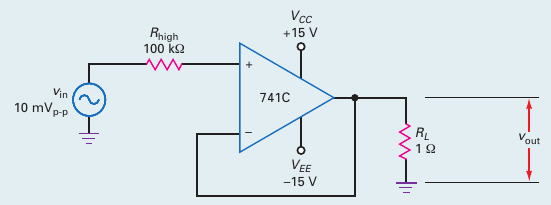
\includegraphics[width=\linewidth]{gambar/fig-16.26a}
	\end{center}
	\columnbreak
	\begin{itemize}
		\item Pertanyaan:
		\begin{itemize}
			\item Berapa tegangan output dan bandwidth?
		\end{itemize}
		\item Jawaban:
		\begin{itemize}
			\item Penguatan tegangan closed-loopnya adalah unity, sehingga:
			\[ v_{out} = A_{v(CL)} v_{in} = 1(10 \text{ mV}_\text{p-p})\]
			\item Bandwidthnya adalah:
			\[ f_{2(CL)} = f_{unity} = 1 \text{ MHz} \]
		\end{itemize}
	\end{itemize}
\end{multicols}
\end{frame}

\subsection{Latihan Soal 2.13}
\begin{frame}{Latihan Soal 2.13}
	\begin{multicols}{2}
		\begin{center}
			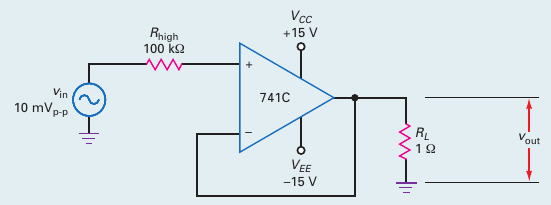
\includegraphics[width=\linewidth]{gambar/fig-16.26a}
		\end{center}
		\columnbreak
		\begin{itemize}
			\item Pertanyaan:
			\begin{itemize}
				\item Berapa tegangan output dan bandwidth jika op amp yang digunakan adalah LF157A?
			\end{itemize}
		\end{itemize}
	\end{multicols}
\end{frame}

\subsection{Contoh Soal 2.14}
\begin{frame}{Contoh Soal 2.14}
	\begin{multicols}{2}
		\begin{center}
			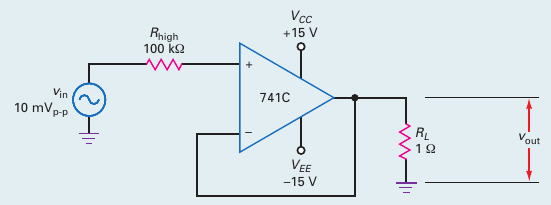
\includegraphics[width=\linewidth]{gambar/fig-16.26a}
		\end{center}
		\columnbreak
		\begin{itemize}
			\item Pertanyaan:
			\begin{itemize}
				\item Jika rangkaian voltage follower di samping dibuat dengan Multisim, tegangan output di $ 1 ~\Omega $ adalah $ 9.99 \text{ mV} $. Tentukan berapa impedansi output closed-loop?
			\end{itemize}
		\end{itemize}
	\end{multicols}
\end{frame}

\begin{frame}{Contoh Soal 2.14}
	\begin{multicols}{2}
		\begin{center}
			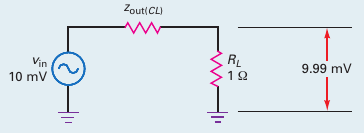
\includegraphics[width=\linewidth]{gambar/fig-16.26b}
		\end{center}
		\columnbreak
		\begin{itemize}
			\item Jawaban:
			\begin{itemize}
				\item Tegangan output:
				\[  v_{out} = 9.99 \text{ mV}  \]
				\item Arus di beban adalah:
				\[ i_{out} = \frac{9.99 \text{ mV}}{1~\Omega} = 9.99 \text{ mA} \]
				\item Impedansi output closed-loop
				\[ z_{out(CL)} = \frac{0.01 \text{ mV}}{9.99 \text{ mA}} = 0.001~\Omega \]
			\end{itemize}
		\end{itemize}
	\end{multicols}
\end{frame}

\subsection{Latihan Soal 2.14}
\begin{frame}{Latihan Soal 2.14}
	\begin{multicols}{2}
		\begin{center}
			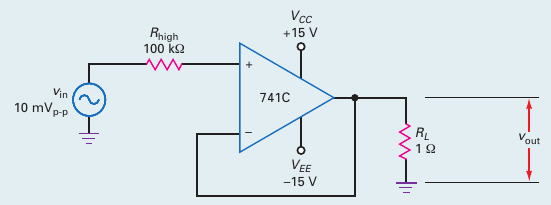
\includegraphics[width=\linewidth]{gambar/fig-16.26a}
		\end{center}
		\columnbreak
		\begin{itemize}
			\item Pertanyaan:
			\begin{itemize}
				\item Jika rangkaian voltage follower di samping dibuat dengan Multisim, tegangan output di $ 1 ~\Omega $ adalah $ 9.95 \text{ mV} $. Tentukan berapa impedansi output closed-loop?
			\end{itemize}
		\end{itemize}
	\end{multicols}
\end{frame}

\subsection{Ringkasan}
\begin{frame}{Ringkasan}
	\begin{center}
		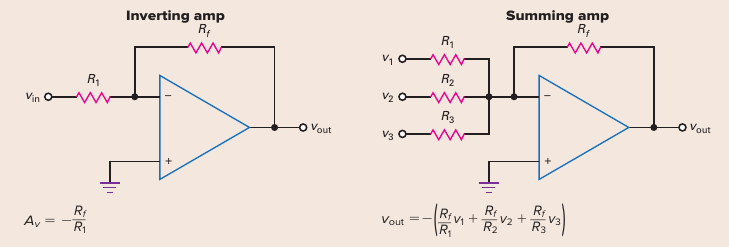
\includegraphics[width=\linewidth]{gambar/table-16.2a}
	\end{center}
\end{frame}

\begin{frame}{Ringkasan}
	\begin{center}
		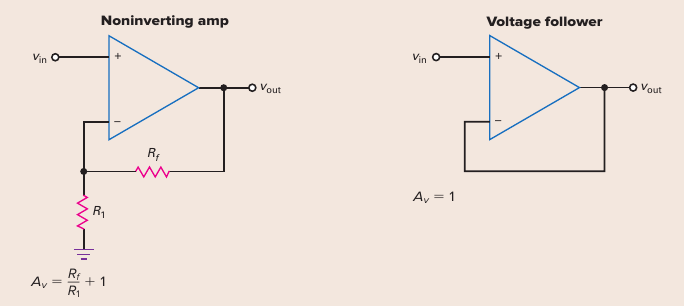
\includegraphics[width=\linewidth]{gambar/table-16.2b}
	\end{center}
\end{frame}